\section{Platform Demo and Problem Context}

% ============================================================
% S2: LIVE PLATFORM DEMO - CONFIGURATION
% ============================================================
\begin{frame}{Live Platform Demo: Evaluation Configuration}
    \begin{columns}[T]
        \begin{column}{0.48\textwidth}
            \begin{itemize}
                \item MEDF evaluates AI systems against multiple governance frameworks simultaneously.
                \item Configurable stakeholder weights model different value systems.
                \item Live at: {\footnotesize\url{https://ccds25-0582-medf-api.streamlit.app/}}.
            \end{itemize}
        \end{column}
        \begin{column}{0.48\textwidth}
            \centering
            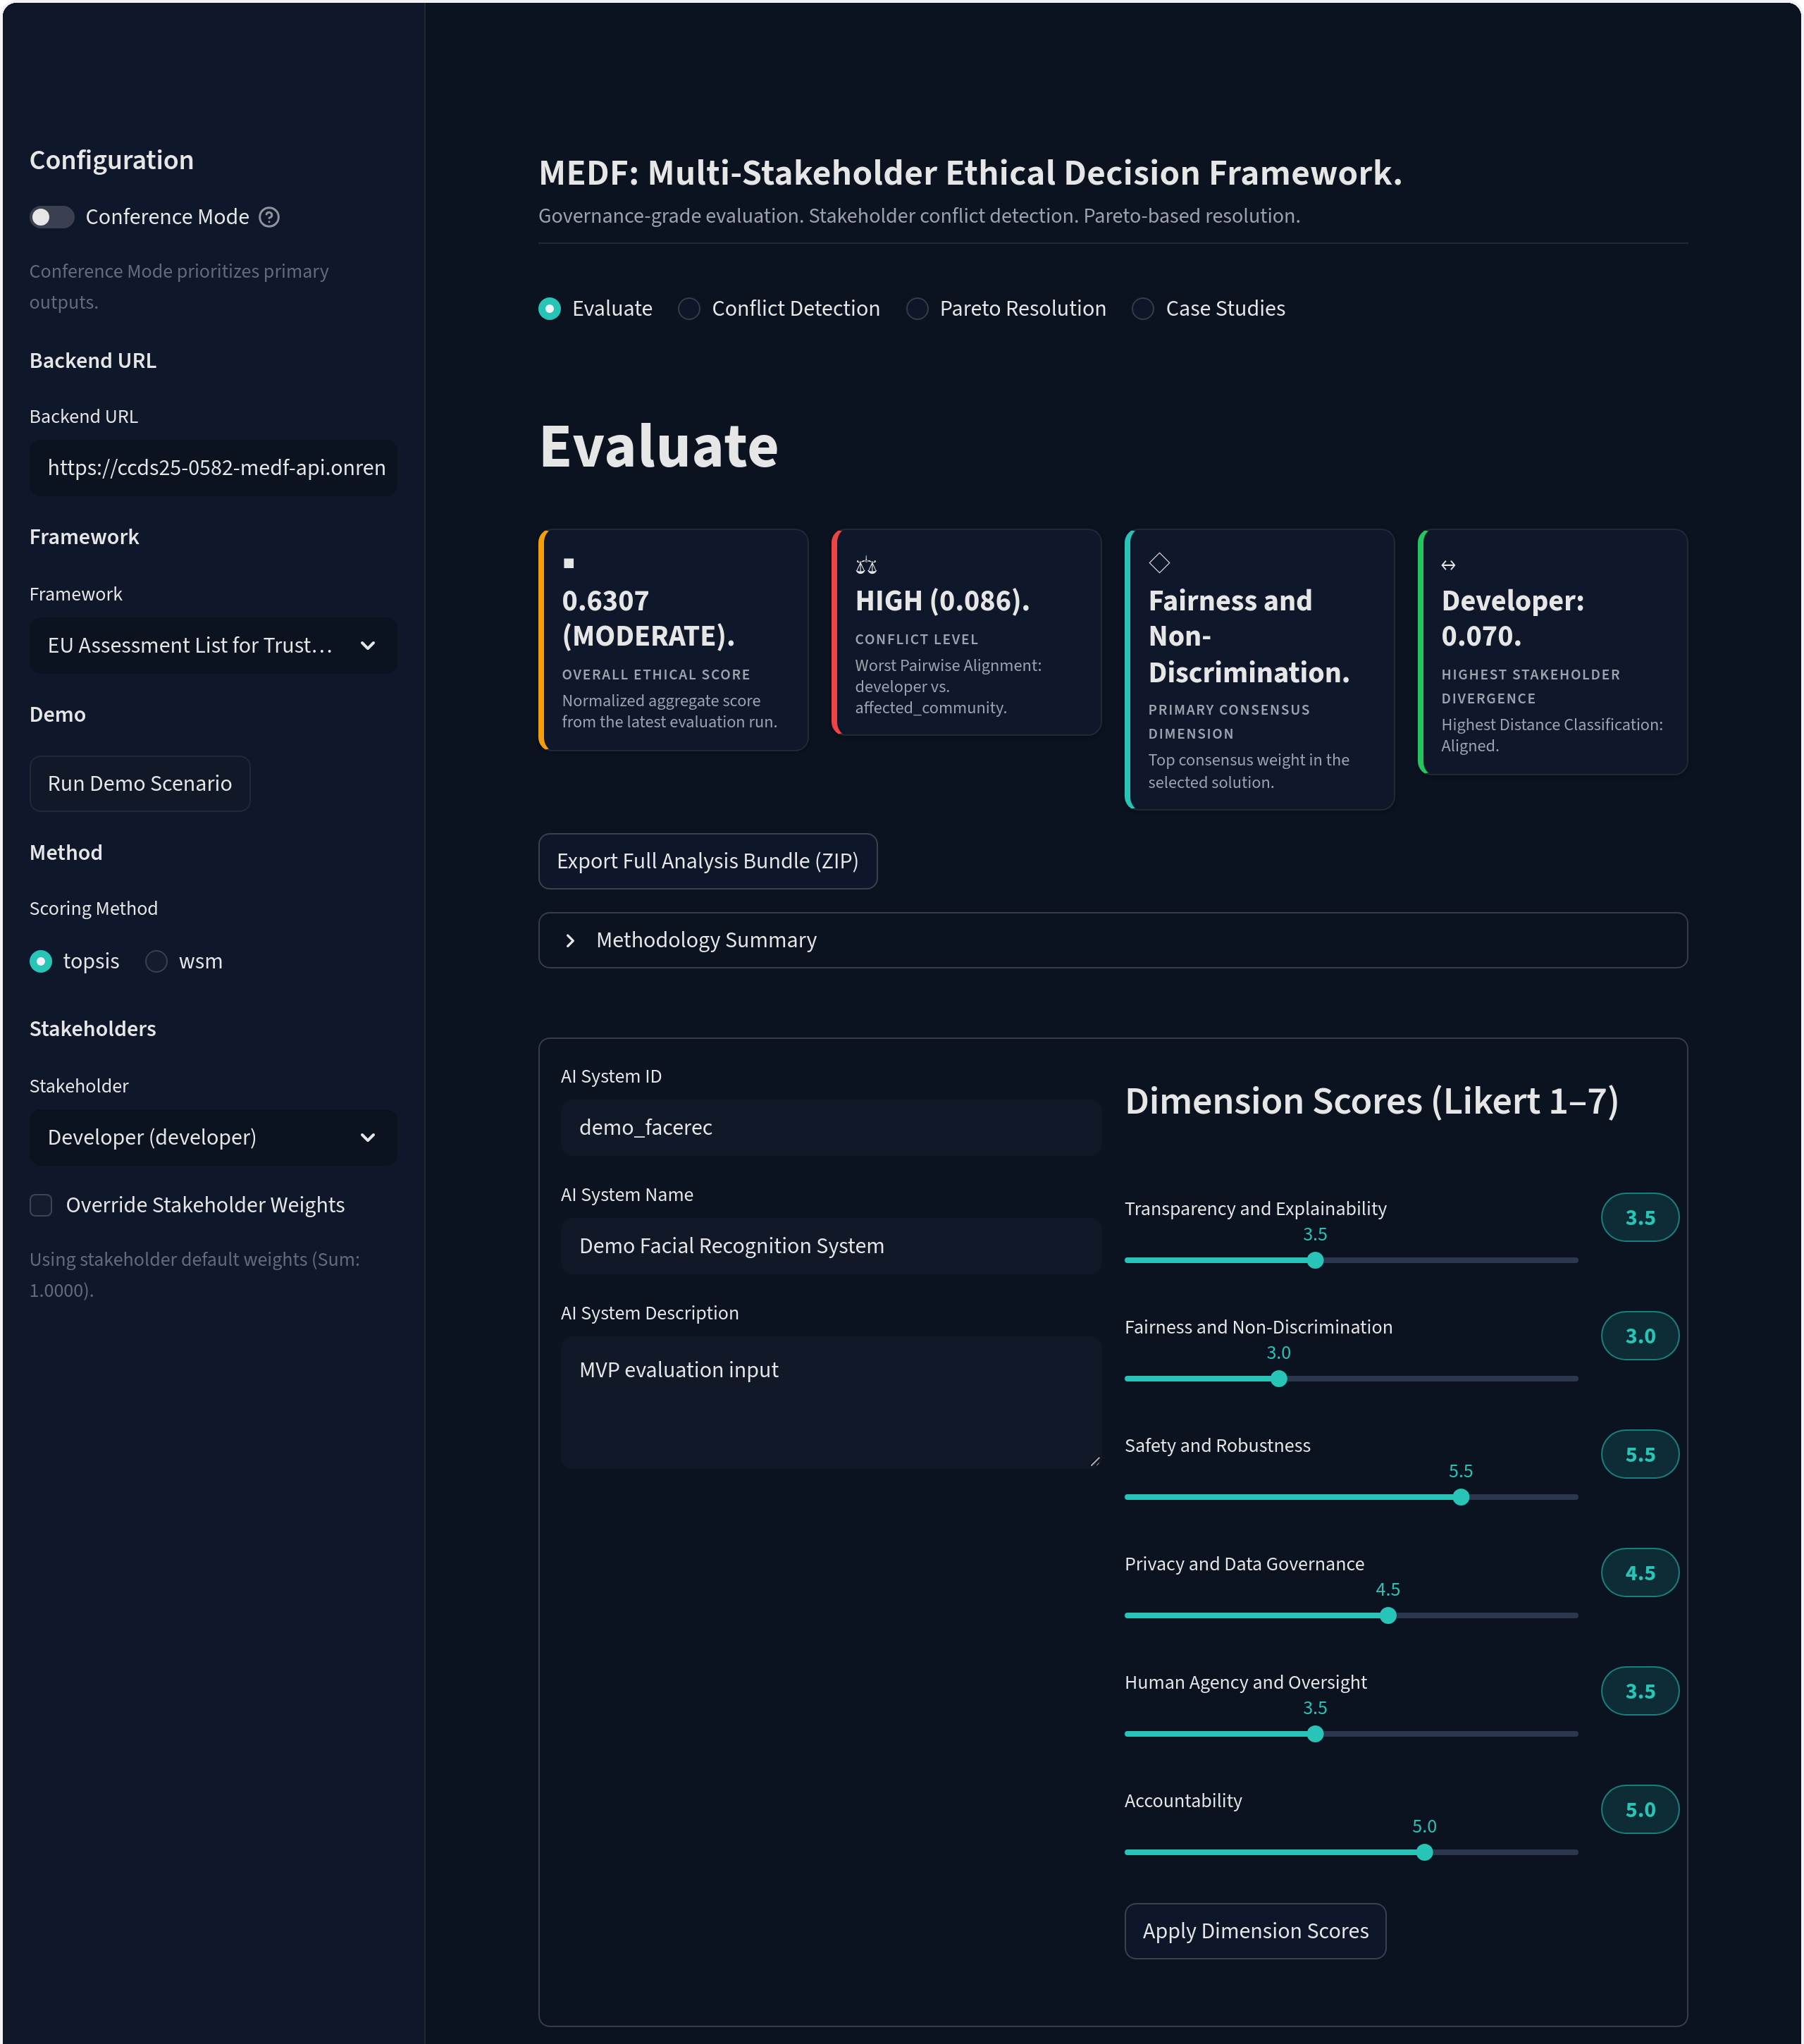
\includegraphics[width=\linewidth,height=0.55\textheight,keepaspectratio]{images/fig_10_1_config.png}

            {\footnotesize Figure 10.1: MEDF evaluation configuration interface.}
        \end{column}
    \end{columns}
\end{frame}
% NOTES: Walk the audience through the interface. Point out the dimension score sliders,
% framework selector and stakeholder dropdown. Approximately 60 seconds.
% Transition: "When we run this evaluation, here is what the results look like."

% ============================================================
% S3: DEMO - RESULTS VISUALIZATION
% ============================================================
\begin{frame}{Demo: Evaluation Results}
    \begin{columns}[T]
        \begin{column}{0.48\textwidth}
            \begin{itemize}
                \item Overall ethical score with risk classification (Low, Medium, High, Critical).
                \item Radar chart reveals dimensional strengths and weaknesses.
                \item Per-framework breakdown shows regulatory perspective differences.
            \end{itemize}
        \end{column}
        \begin{column}{0.48\textwidth}
            \centering
            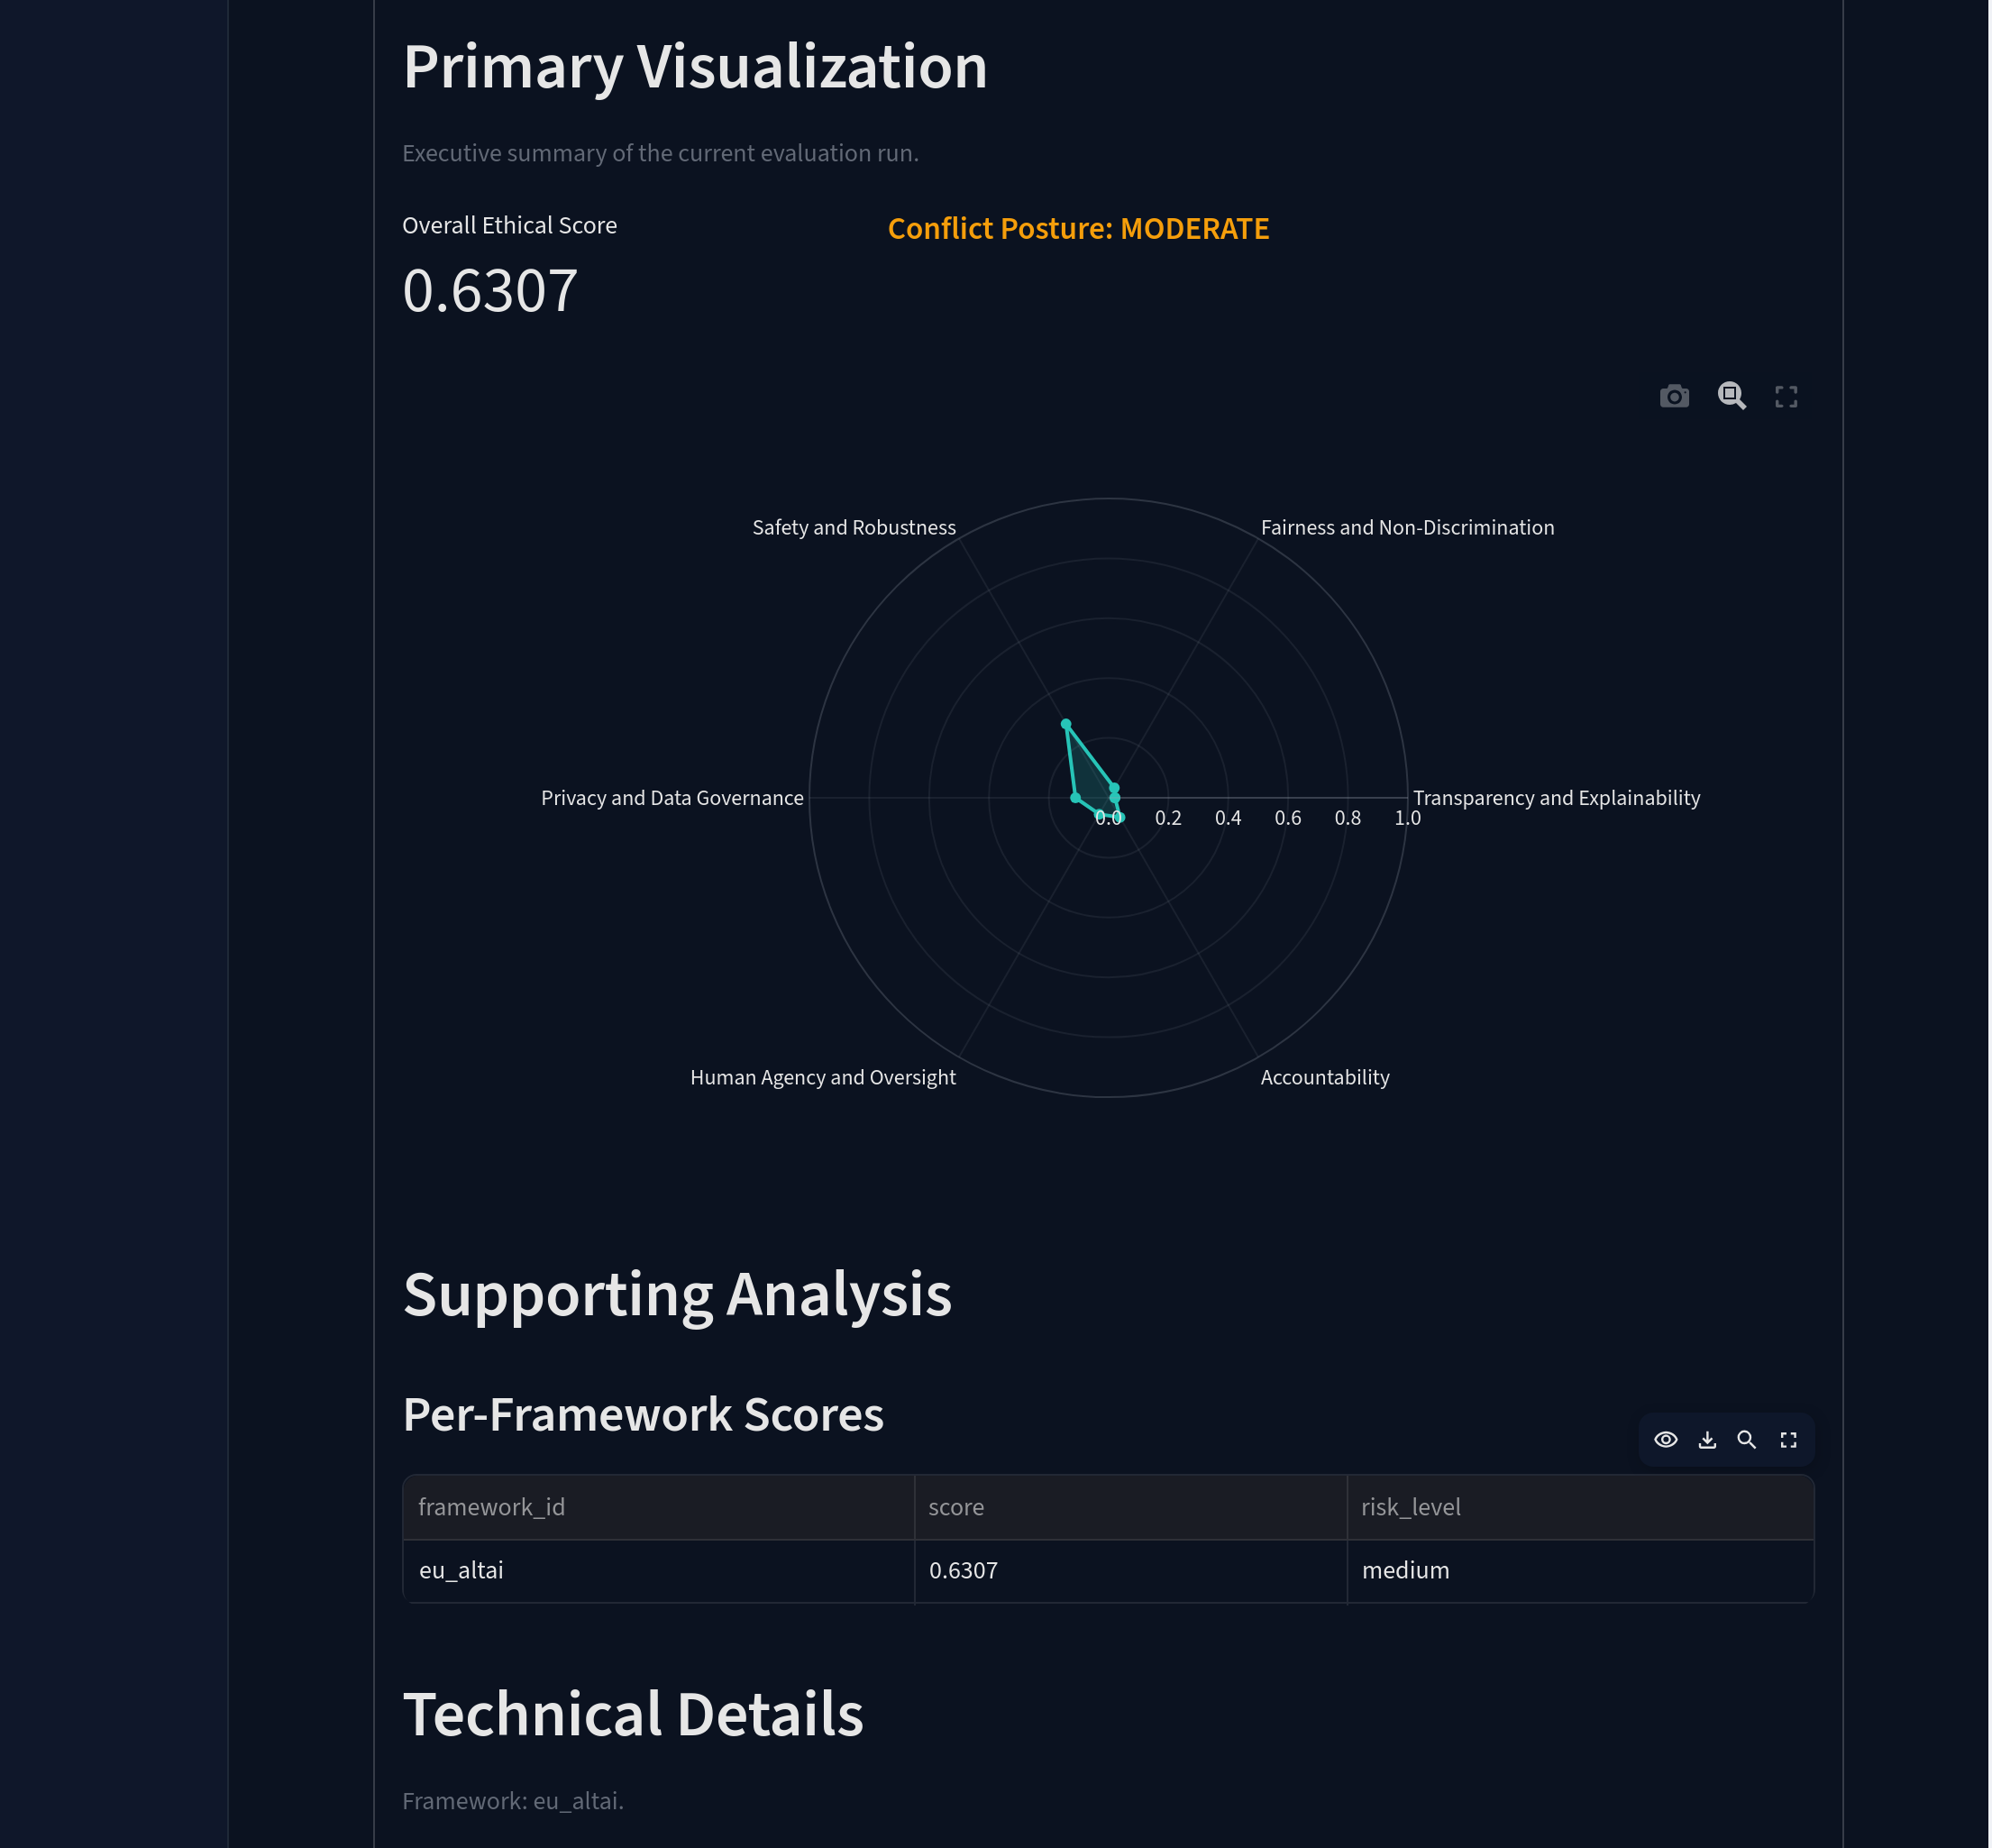
\includegraphics[width=\linewidth,height=0.55\textheight,keepaspectratio]{images/fig_10_2_results.png}

            {\footnotesize Figure 10.2: MEDF evaluation results visualization.}
        \end{column}
    \end{columns}
\end{frame}
% NOTES: Highlight the radar chart shape and the score gauge. Explain that the same
% system scores differently under different frameworks. Approximately 30 seconds.
% Transition: "The platform also detects conflicts between stakeholders."

% ============================================================
% S4: DEMO - CONFLICT AND PARETO
% ============================================================
\begin{frame}{Demo: Conflict Detection and Pareto Resolution}
    \begin{columns}[T]
        \begin{column}{0.48\textwidth}
            \centering
            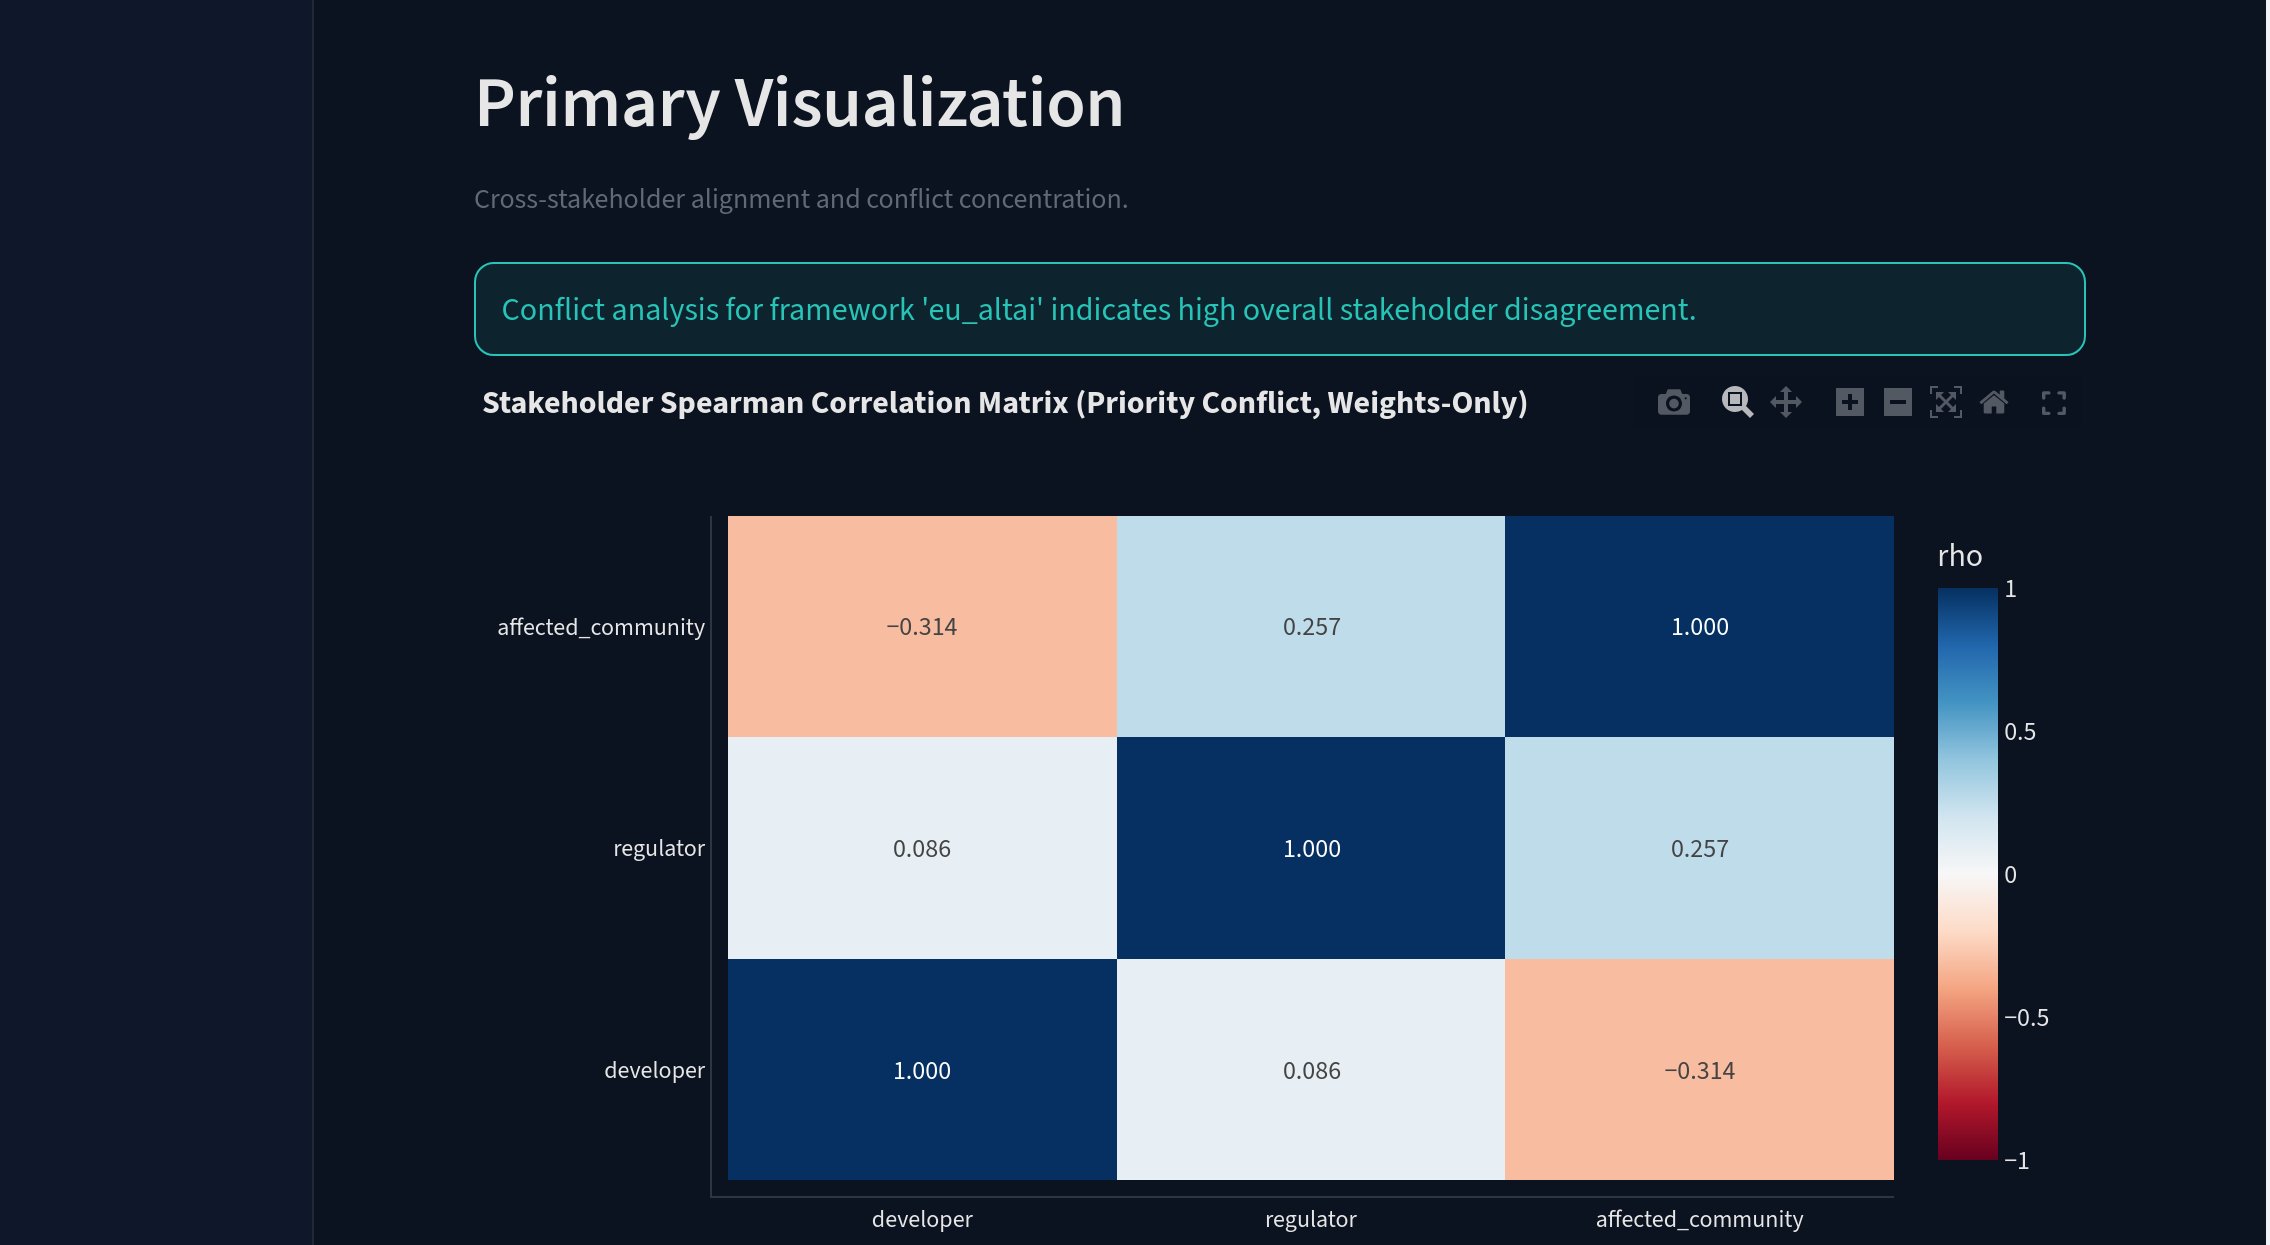
\includegraphics[width=\linewidth,height=0.55\textheight,keepaspectratio]{images/fig_10_3_conflict.png}

            {\footnotesize Figure 10.3: Conflict detection heatmap (Spearman $\rho$).}
        \end{column}
        \begin{column}{0.48\textwidth}
            \centering
            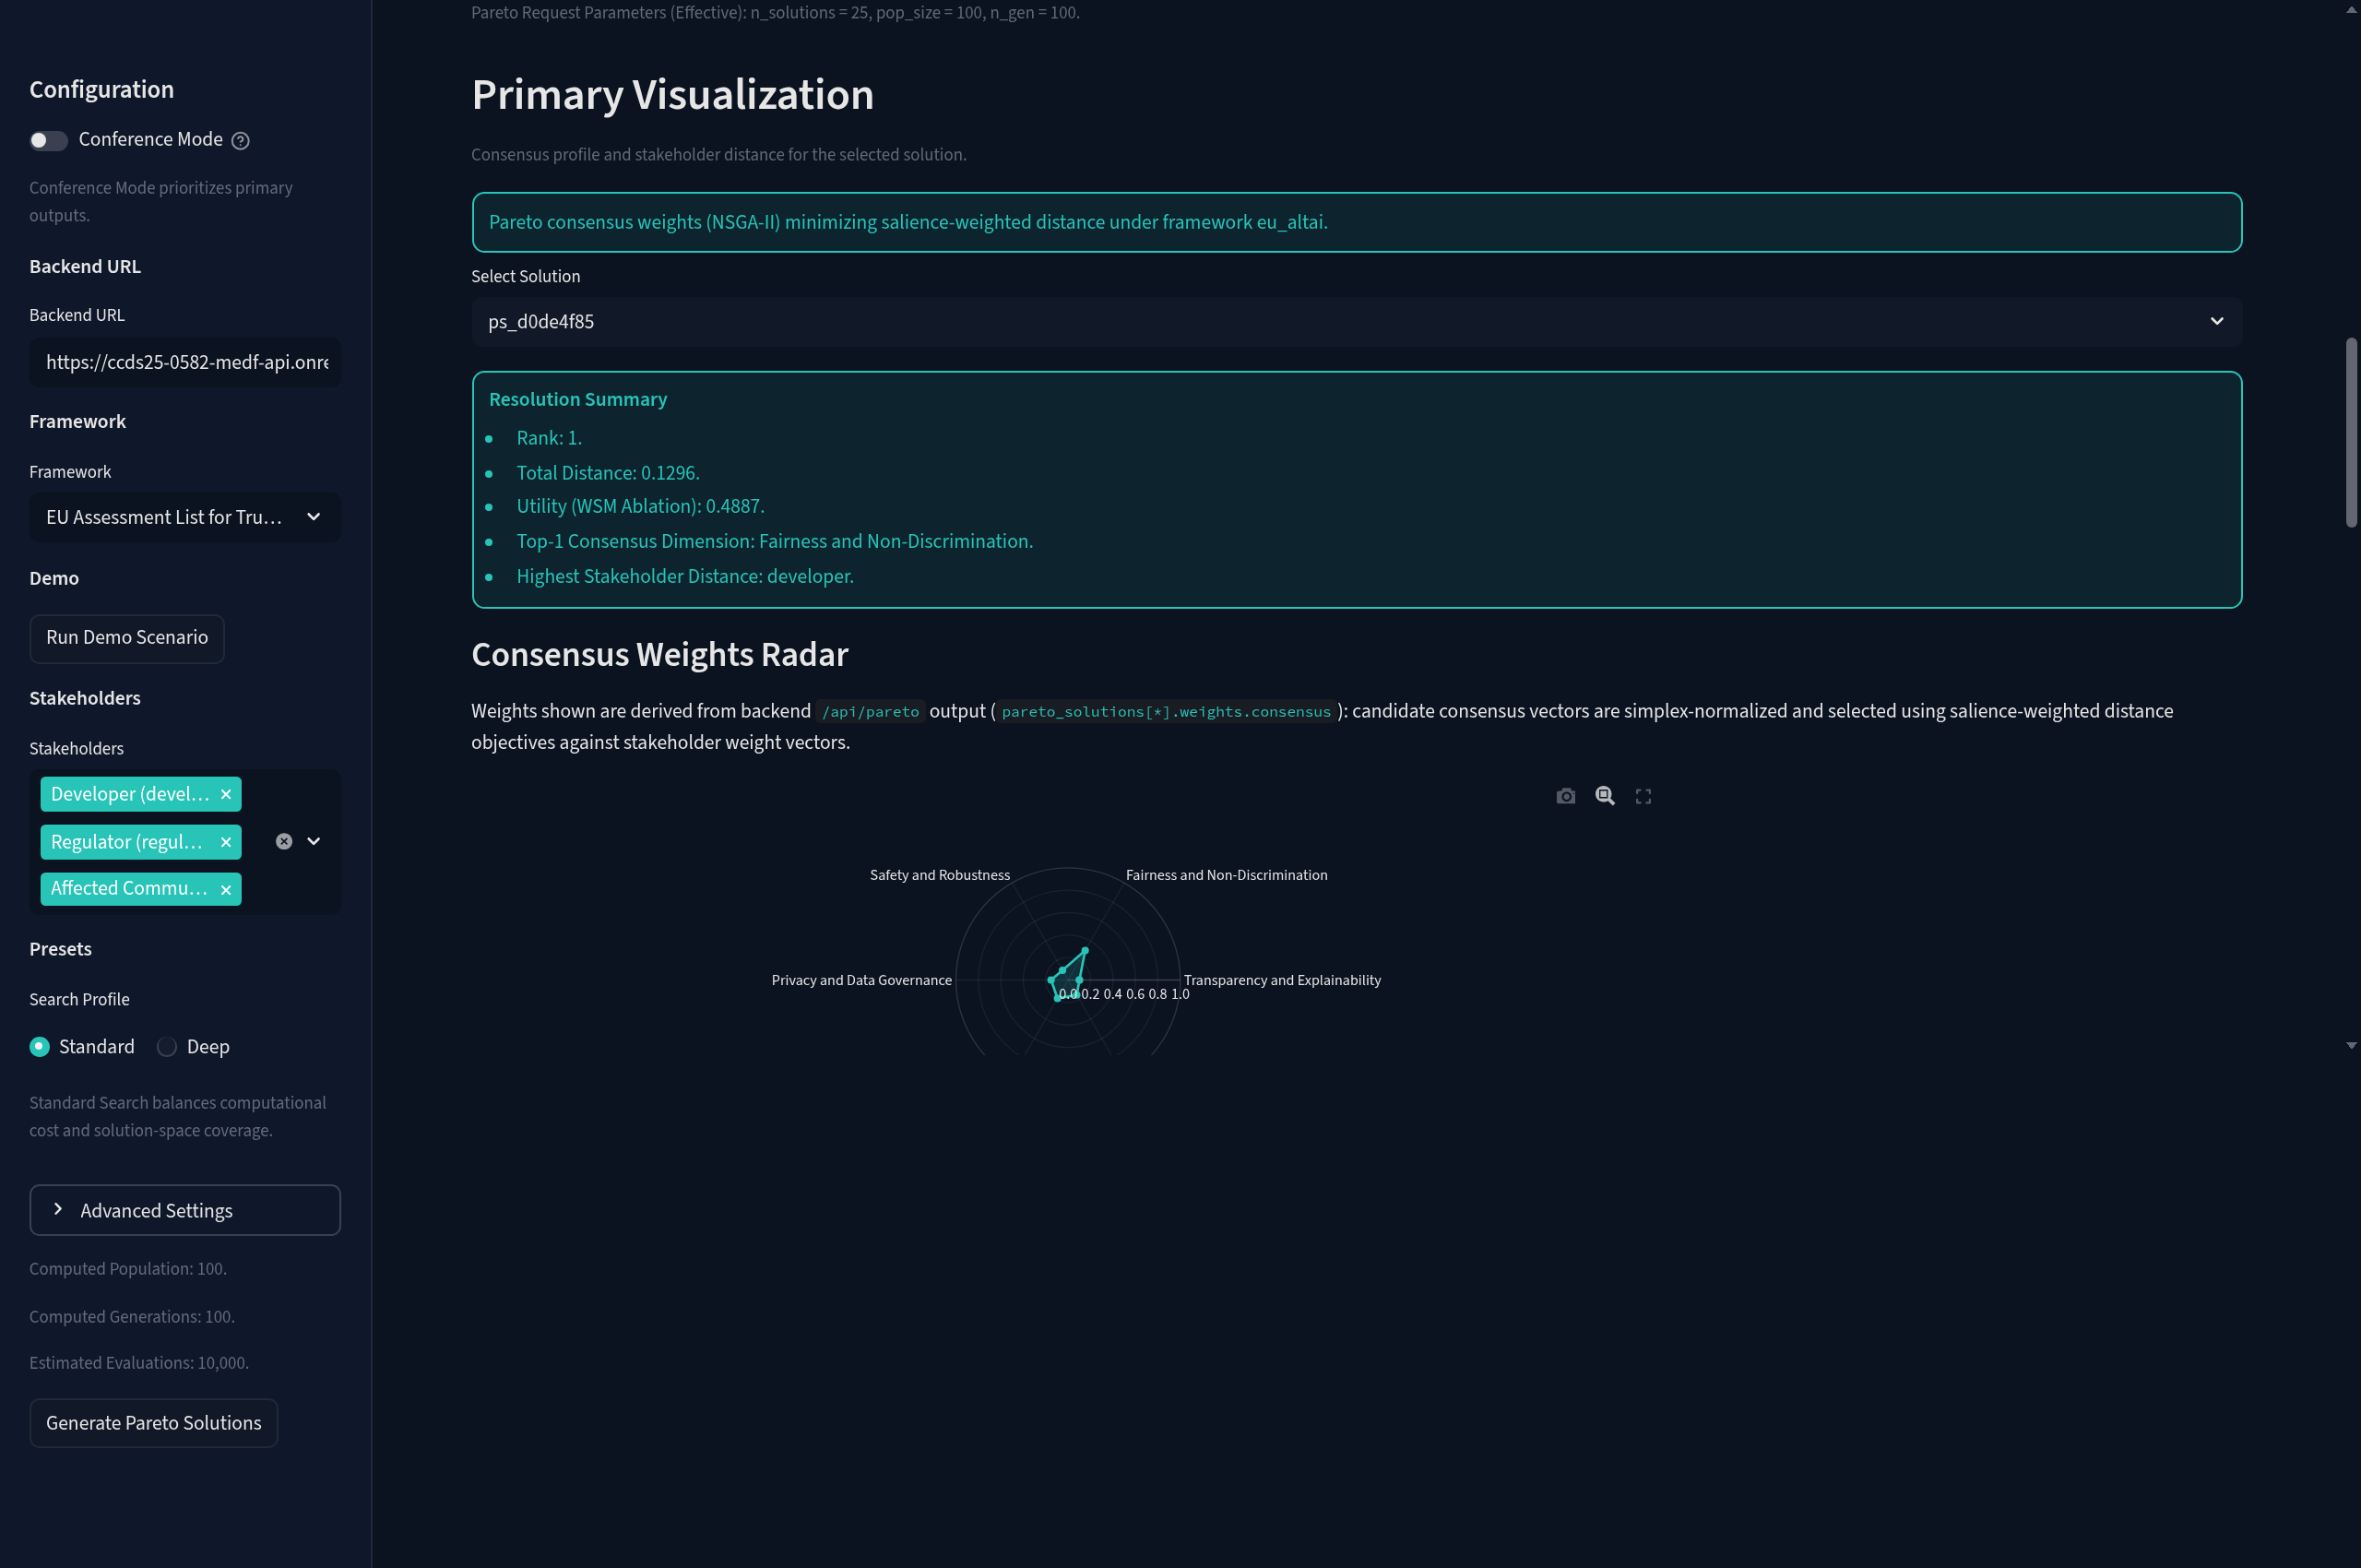
\includegraphics[width=\linewidth,height=0.55\textheight,keepaspectratio]{images/fig_10_4_pareto.png}

            {\footnotesize Figure 10.4: Pareto resolution consensus solutions.}
        \end{column}
    \end{columns}
\end{frame}
% NOTES: Left panel shows where stakeholders agree and disagree. Right panel shows
% NSGA-II generated compromise weight vectors. Approximately 30 seconds.
% Transition: "Now let me provide the context for why this platform was built."

% ============================================================
% S5: OUTLINE
% ============================================================
\begin{frame}{Outline}
    \begin{enumerate}
        \item Platform Demo \textcolor{gray}{(completed)}.
        \item Problem Definition and Gap Analysis.
        \item Methodology, Architecture, and Algorithms.
        \item Case Study Evaluation.
        \item Limitations, Future Work, and Contributions.
    \end{enumerate}
\end{frame}
% NOTES: Brief orientation slide. Approximately 15 seconds.
% Transition: "Let me start with the problem this project addresses."

% ============================================================
% S6: PROBLEM AND MOTIVATION
% ============================================================
\begin{frame}{Problem and Motivation}
    \textbf{Three Interconnected Sub-Problems in AI governance:}
    \begin{enumerate}
        \item \textbf{No standardized metrics.} Ethical concepts remain abstract and context-dependent, making evaluations subjective and incomparable~\cite{mittelstadt2019principles}.
        \item \textbf{Unmanaged stakeholder conflict.} Developers, regulators, and affected communities hold divergent priorities~\cite{freeman1984strategic, mitchell1997stakeholder}.
        \item \textbf{No auditable workflows.} Ethical assessments lack traceability and reproducibility~\cite{hagendorff2020ethics}.
    \end{enumerate}

    \vspace{6pt}
    \textit{Real-World Failures:} facial recognition bias~\cite{buolamwini2018gender}, iTutorGroup age discrimination~\cite{eeoc2022itutorgroup}, NHS-DeepMind privacy breach~\cite{ico2017deepmind}. These patterns are systemic~\cite{oneil2016weapons, raji2020closing}.
\end{frame}
% NOTES: Emphasize these are not hypothetical problems. Each example led to regulatory
% action or public controversy. Approximately 75 seconds.
% Anticipated question: "Why these three sub-problems specifically?"
% Response: "These map directly to the three gaps identified in the literature: Mittelstadt
% showed principles alone fail, Freeman's stakeholder theory shows conflict is structural,
% and Hagendorff found guidelines lack enforcement mechanisms."
% Transition: "No existing tool addresses all three simultaneously."

% ============================================================
% S7: GAP ANALYSIS
% ============================================================
\begin{frame}{Gap Analysis: What Existing Tools Miss}
    \centering
    \footnotesize
    \setlength{\tabcolsep}{3pt}
    \begin{tabular}{l c c c c c c}
        \toprule
        \textbf{Capability} & \textbf{ALTAI} & \textbf{AI Verify} & \textbf{Credo AI} & \textbf{AIF360} & \textbf{Z-Insp.} & \textbf{MEDF} \\
        \midrule
        Cross-framework comparison   & --     & --     & --     & --     & --     & \checkmark \\
        Stakeholder weighting        & --     & --     & --     & --     & --     & \checkmark \\
        Conflict detection           & --     & --     & --     & --     & --     & \checkmark \\
        Pareto consensus             & --     & --     & --     & --     & --     & \checkmark \\
        Quantitative scoring         & --     & \checkmark & \checkmark & \checkmark & --     & \checkmark \\
        Multi-dimensional viz.       & --     & \checkmark & \checkmark & \checkmark & --     & \checkmark \\
        \bottomrule
    \end{tabular}

    \vspace{4pt}
    {\footnotesize Source: Comparative analysis from Chapter~12.3, based on Morley et al.~\cite{morley2020from} and Zicari et al.~\cite{zicari2021zinspection}.}
\end{frame}
% NOTES: This is the novelty defense slide. Stress that MEDF is the only tool offering
% all six capabilities simultaneously. Approximately 60 seconds.
% Anticipated question: "How does MEDF differ from Credo AI?"
% Response: "Credo AI applies separate Policy Packs independently. MEDF compares
% frameworks side-by-side and detects conflicts between stakeholder perspectives,
% which Credo AI does not support."
% Transition: "Let me now describe the methodology behind the platform."
